\documentclass{article}
\usepackage{graphicx}
\title{Quiz System }
\author{Rishabh Jain}
\date{\today}
\begin{document}
\maketitle
The provided Java code constitutes a Quiz project aimed for taking Quiz.
In this project, three Java classes were used: Login, Score, and Quiz. The Login class is responsible for handling the login page, the Score class manages the final score display, and the Quiz class handles the quiz questions and user interactions.
Key functionalities include:
\begin{itemize}
\item Enter Your Name.
\item Give Quiz of 10 questions.
\item Your Total Score.
\end{itemize}
This program provides an interactive GUI for students to perform there Quiz effectively.
\begin{center}
\textbf{1) Login Page}
\end{center}
\begin{figure}[h]
\centering
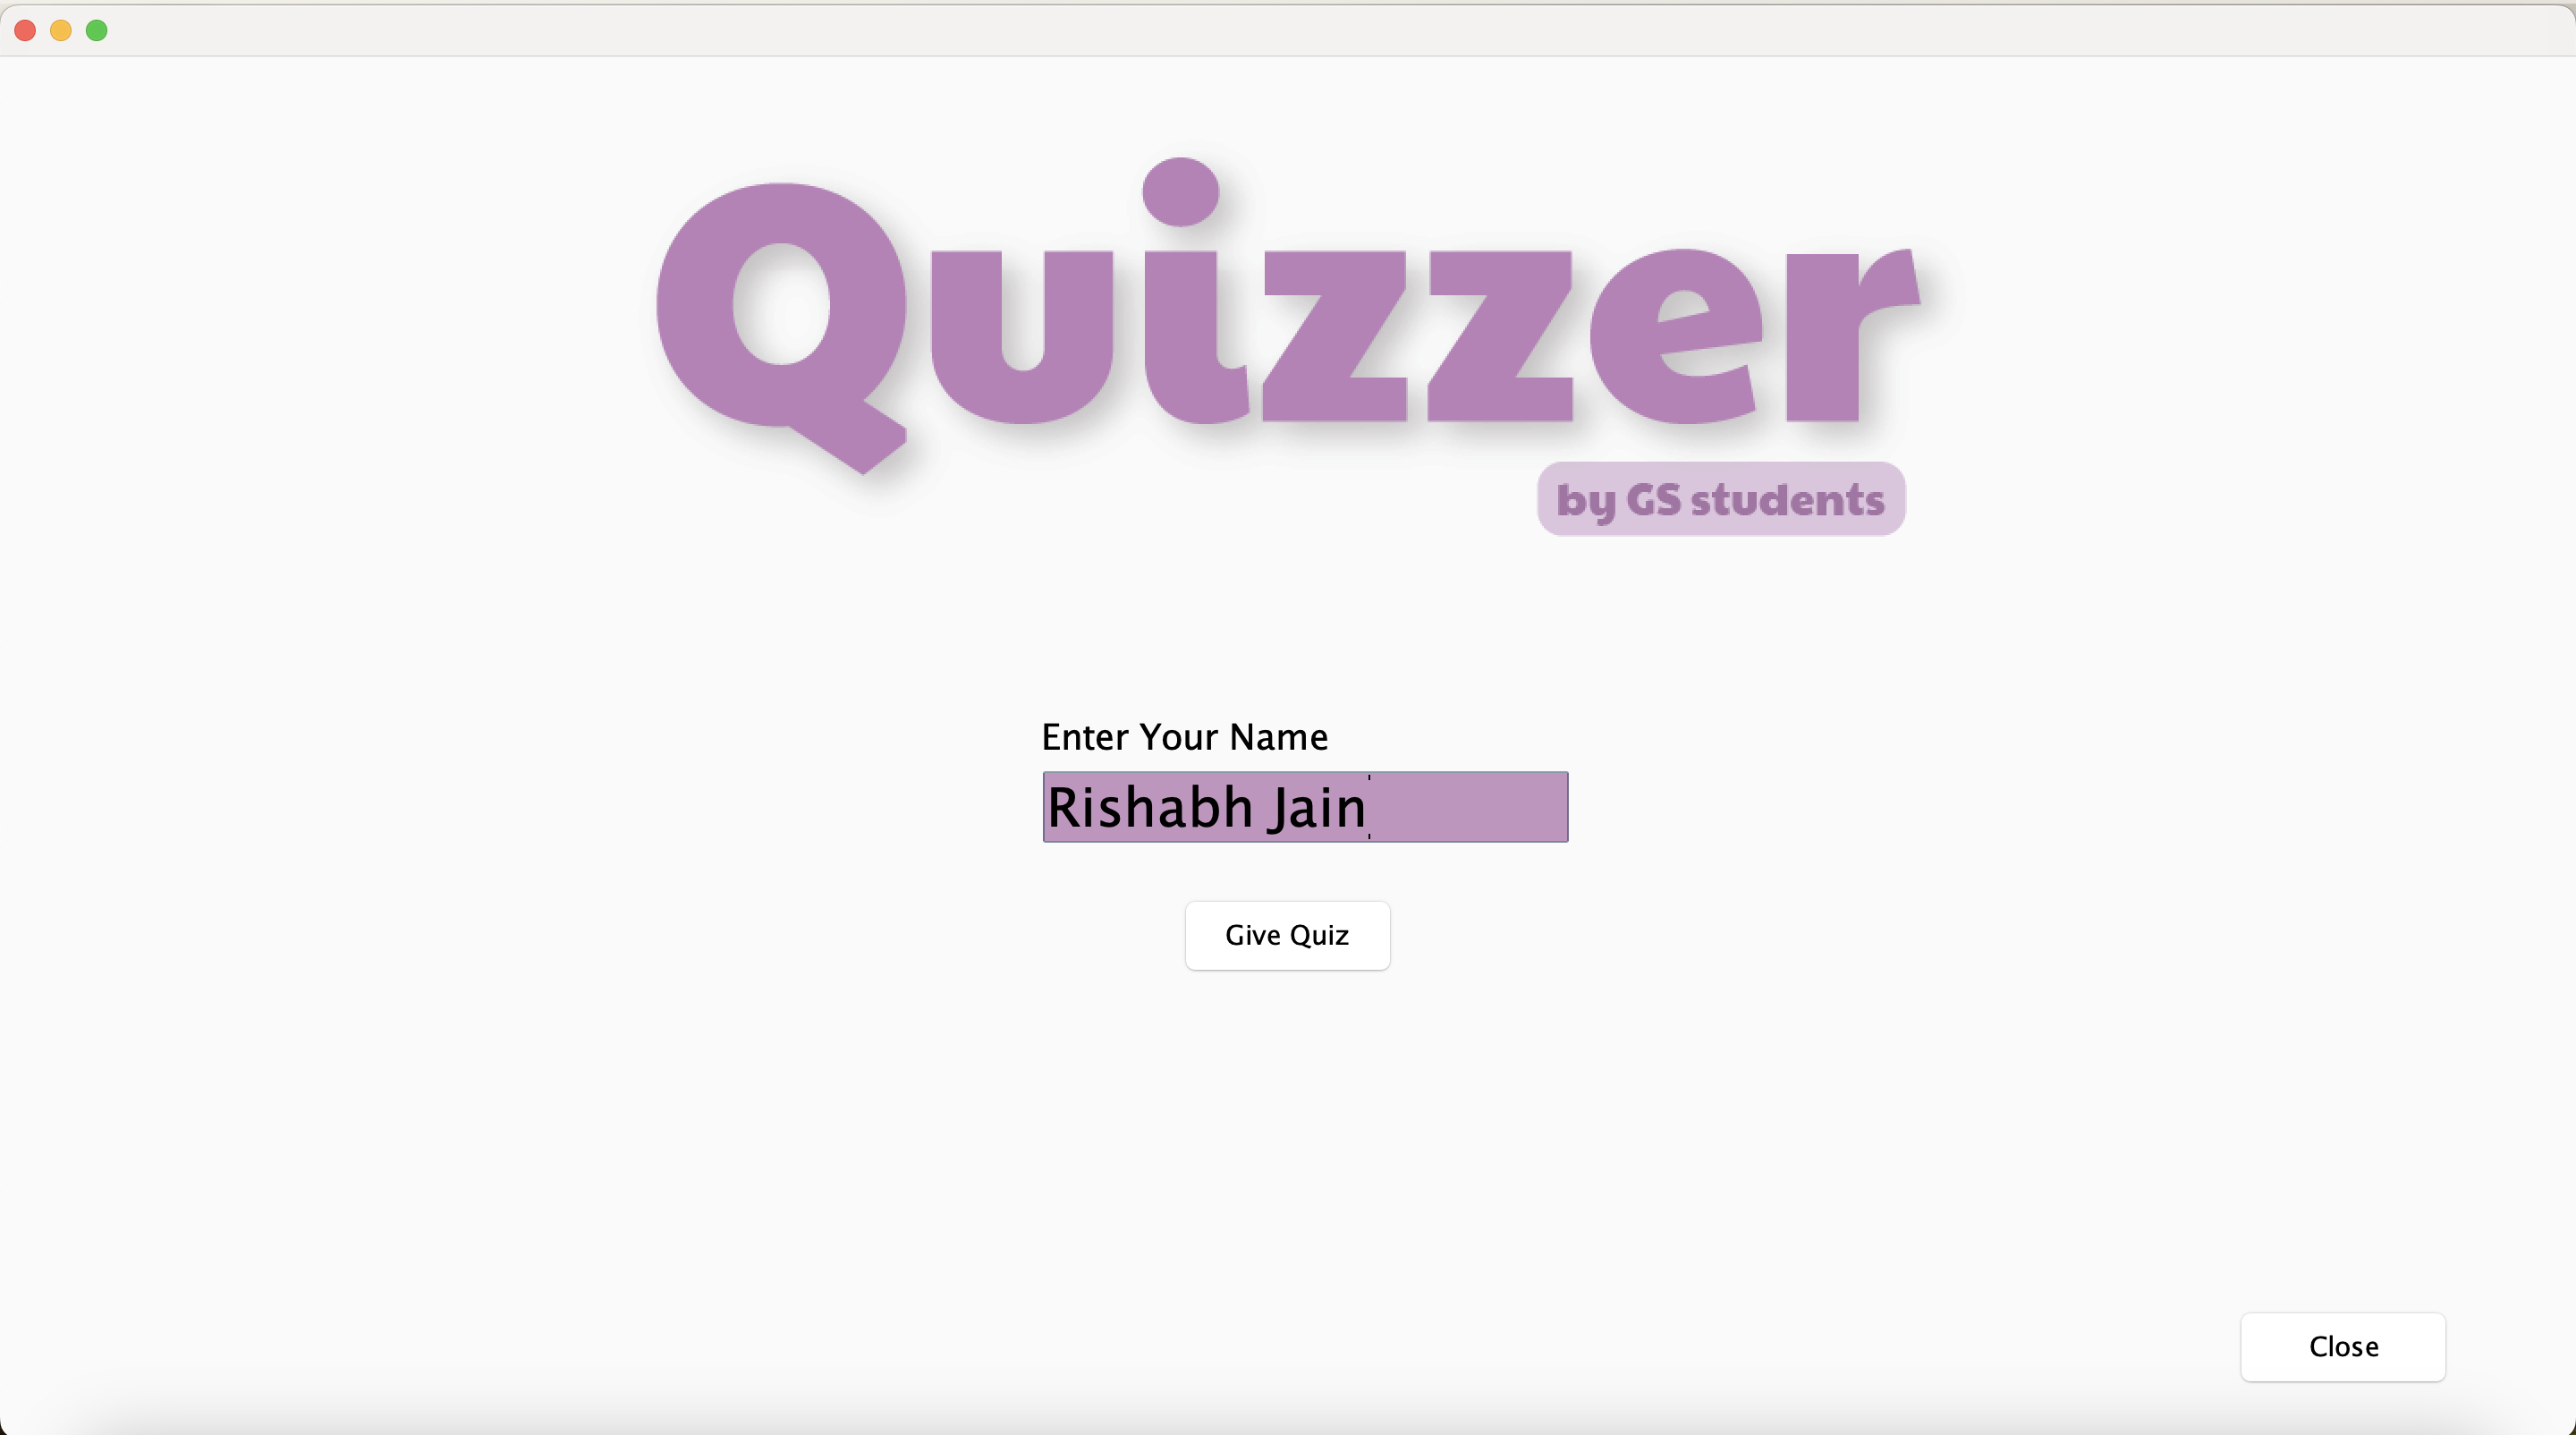
\includegraphics[width=1.0\textwidth]{LoginImage.png}
\label{fig:Login Page}
\end{figure}
\begin{figure}[h]
\begin{center}
\textbf{2) Quiz Questions}
\end{center}
\centering
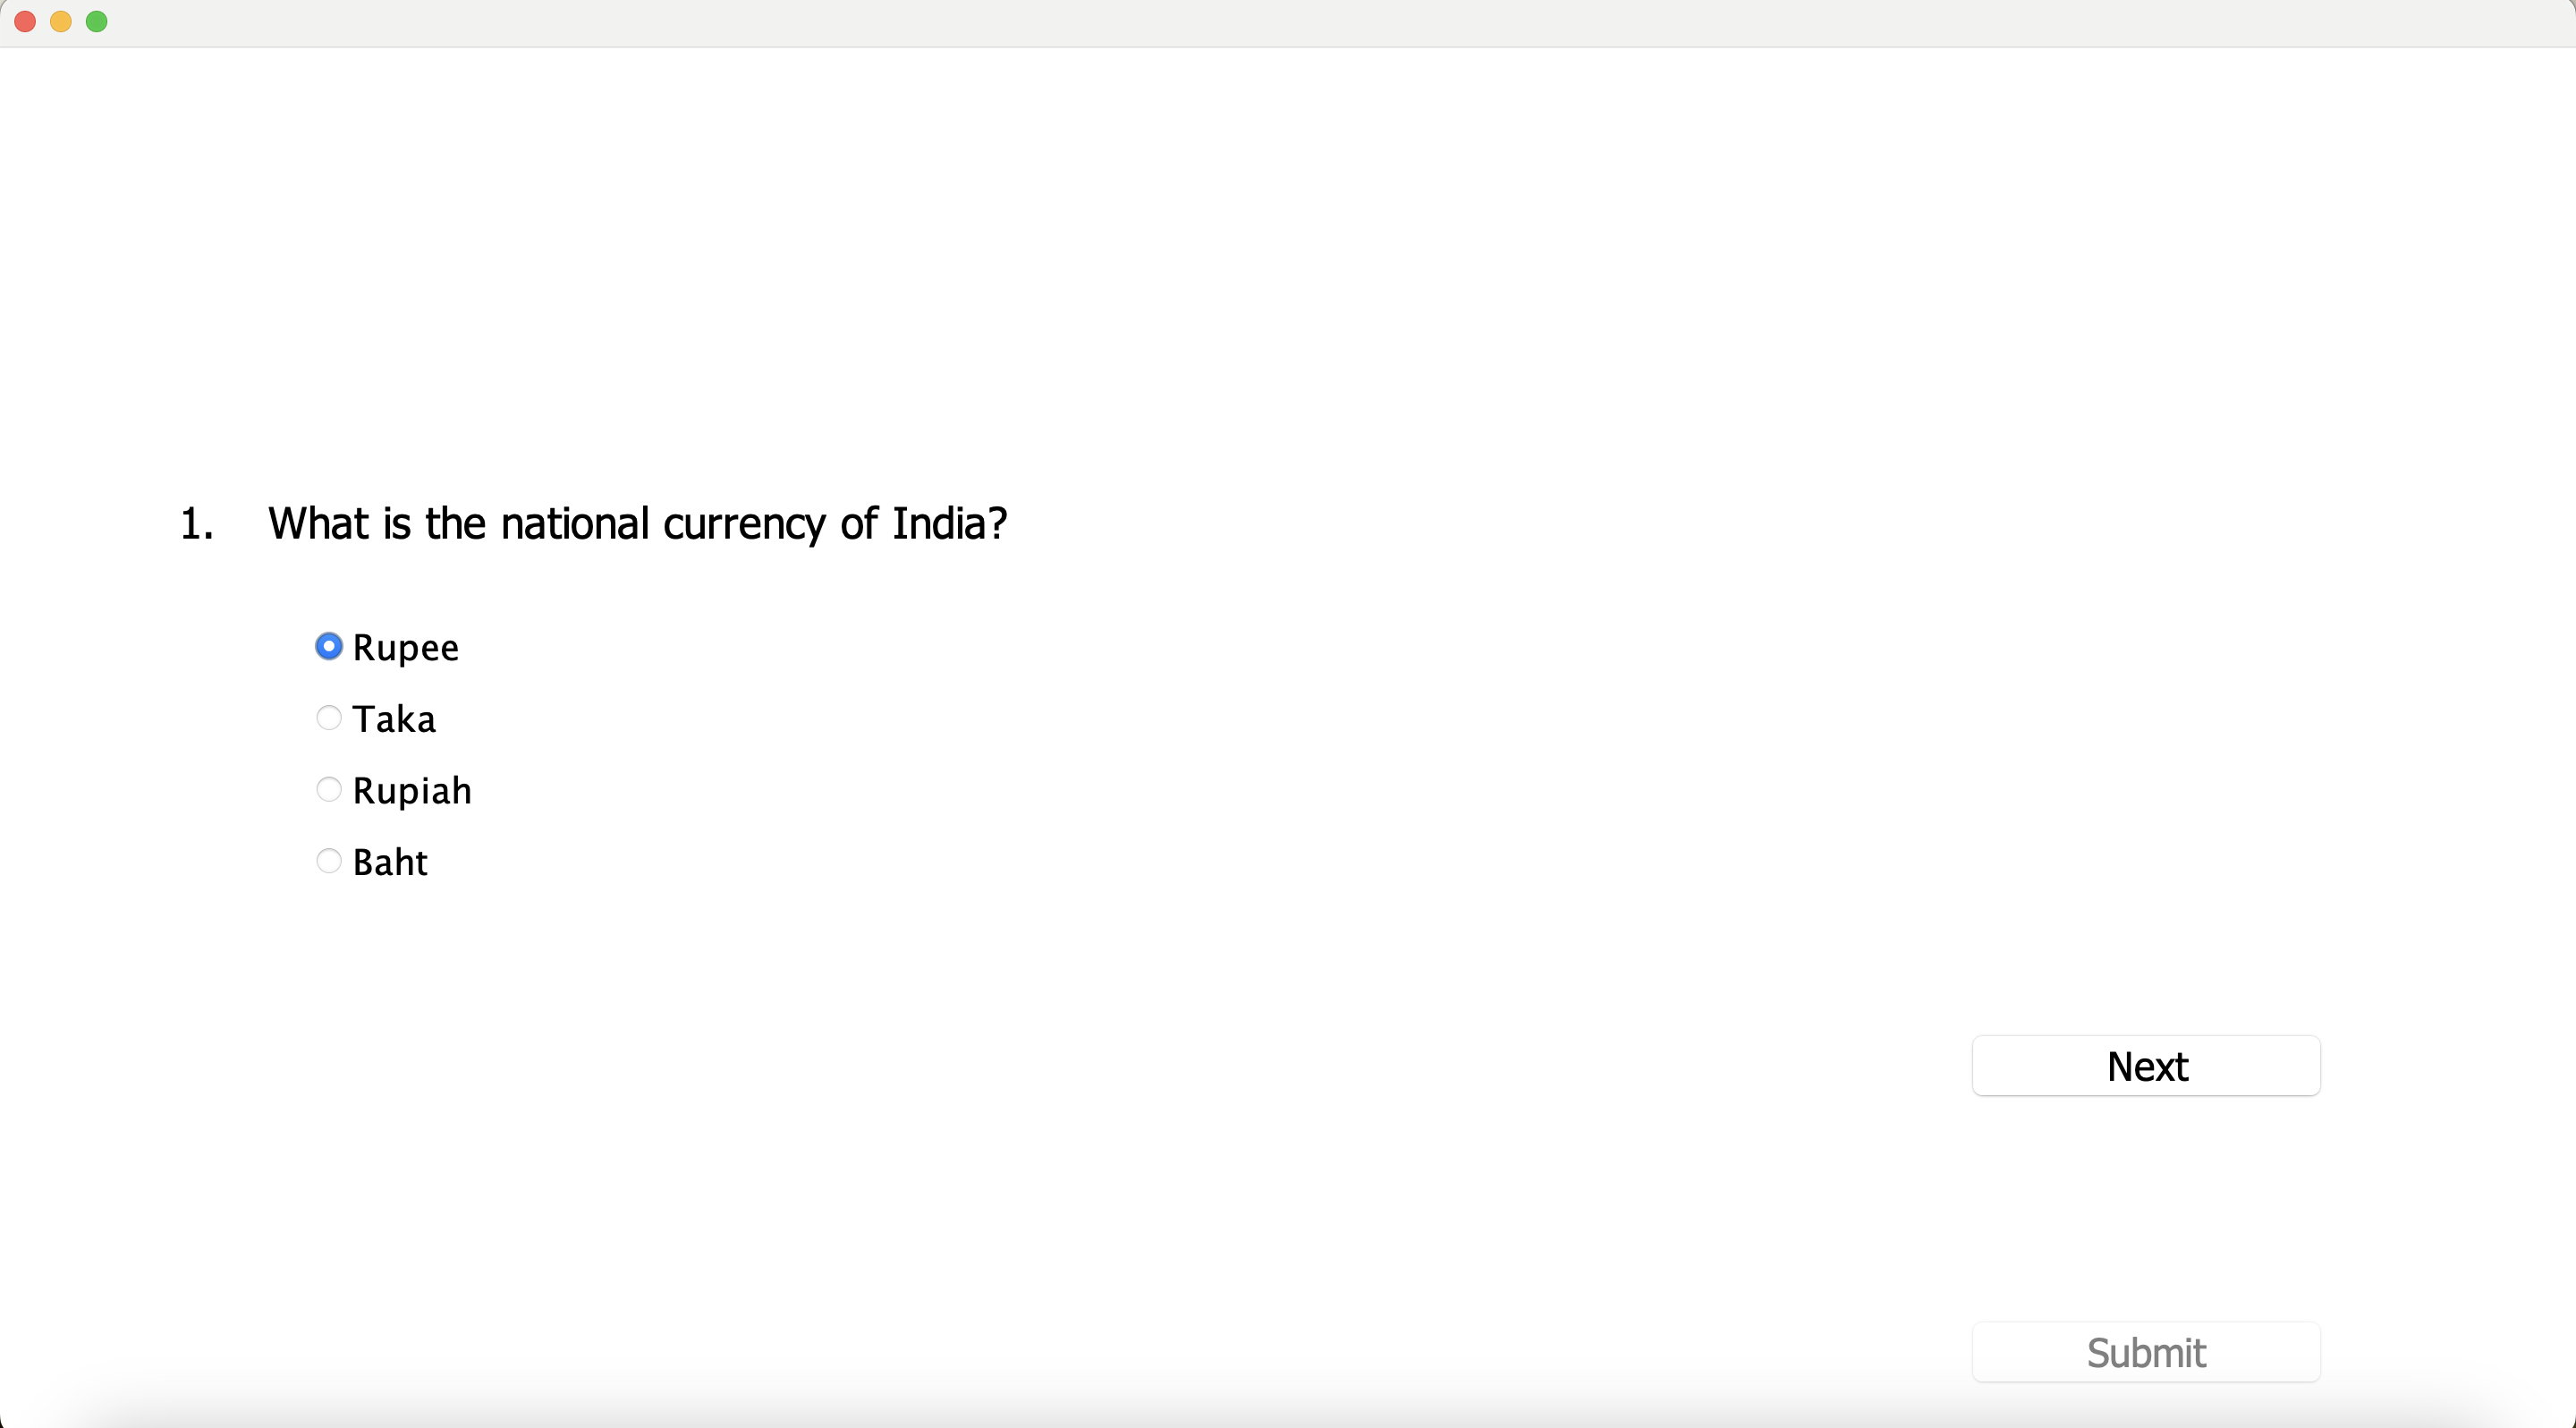
\includegraphics[width=1.0\textwidth]{QuizQue.png}
\label{fig:Quiz Questions}
\end{figure}
\begin{figure}[h]
\begin{center}
\textbf{3)Final Score}
\end{center}
\centering
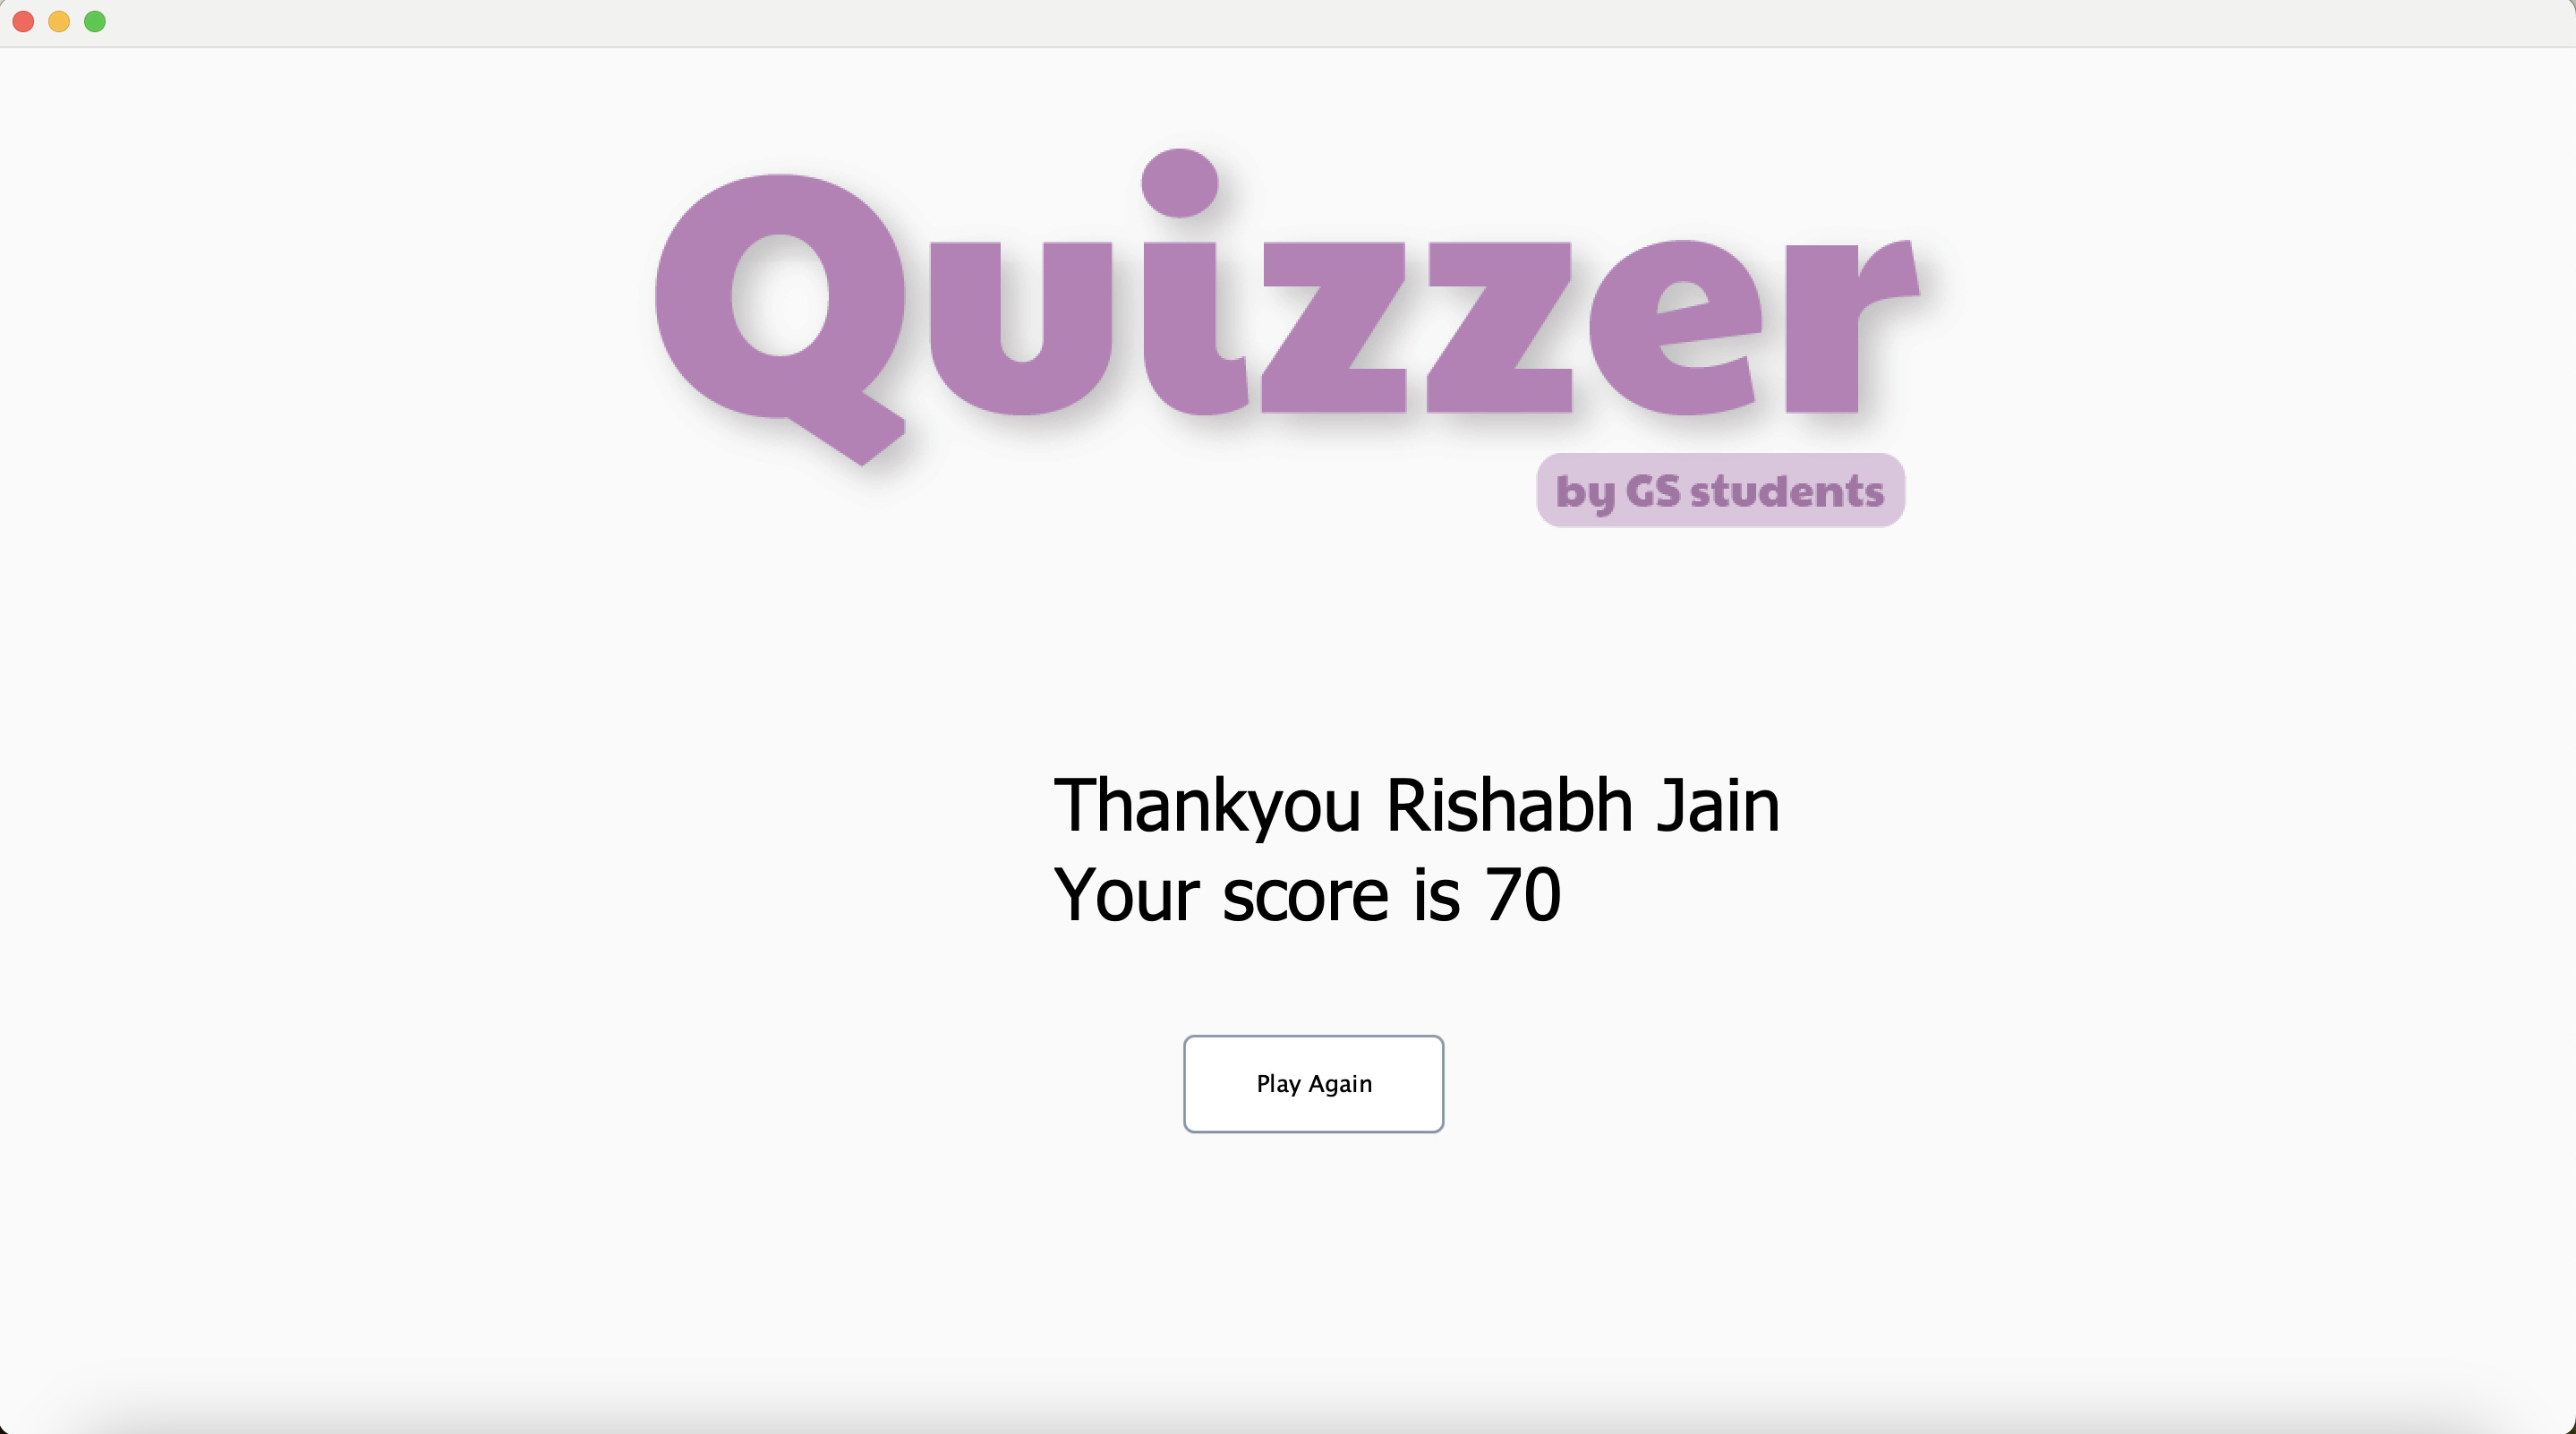
\includegraphics[width=1.0\textwidth]{Score.png}
\label{fig:Score}
\end{figure}
\end{document}